% This is a template file for submitting your homework in math 301. 

\documentclass[letter]{article} %This tells the LaTeX compiler what type of document we are creating

%The next few lines are packages that we load. Geometry allows us to change the margins and other page properties. The amsmath and amssymb packages give us access to common math symbols. 

\usepackage[margin=1in]{geometry}
\usepackage{amsmath}
\usepackage{amssymb}
\usepackage{ifthen}
\usepackage{fancyhdr}
\usepackage{color}
\usepackage[fleqn]{nccmath}
\usepackage{graphicx}
%\graphicspath{ {C:/Users/joh10/Desktop/FSU/CompStat1/Assignments/hw6/} }

%I would like to have space to write comments on your work.  The linespread command below will add extra space to your document.
\linespread{1.5}
 
\pagestyle{fancy}
\rhead{\ifthenelse{\value{page}=1}{\noindent Homework 5 - Weka \hfill Kyle Shaw, Thomas Johansen \\
Oct. 12, 2017 \hfill STA 5635}{Shaw/Johansen}}

\rfoot{\thepage}
\renewcommand{\headrulewidth}{0pt}
\renewcommand{\footrulewidth}{0pt}
\cfoot{}

%We are now ready to start our document.  The next line tells the computer to start creating the PDF. 
\begin{document}
\setlength{\headsep}{0.5 in}
%The section* command below creates an unnumbered section.  If you remove the *, you'll see it numbers the section as section 1. 

\section*{Exploring Classification with Weka}

\quad \quad In this assignment we used the machine learning exploratory tool Weka to compare methods for classification. The dataset Satimage was used, which contains six different classes. We found that SVM had the lowest misclassification error of any of the methods (with the parameter values shown in the table), while still maintaining a fast computation speed. Below is a table of misclassification errrors for train and test sets, as well as runtime for each algorithm. Also included is a plot of test errors vs. computation speed. \\ \\
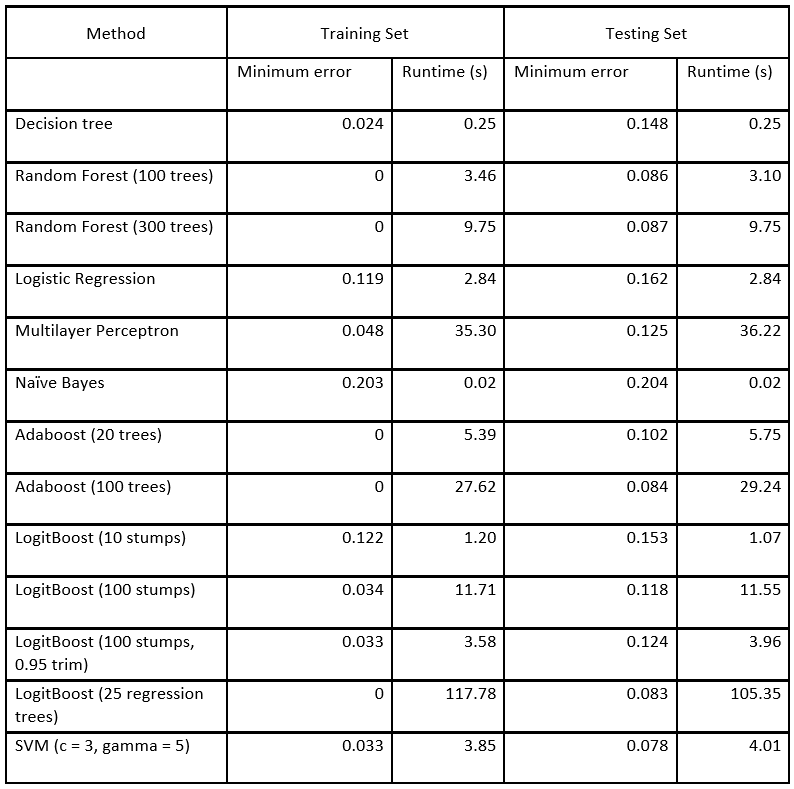
\includegraphics[scale=0.9]{table} \\
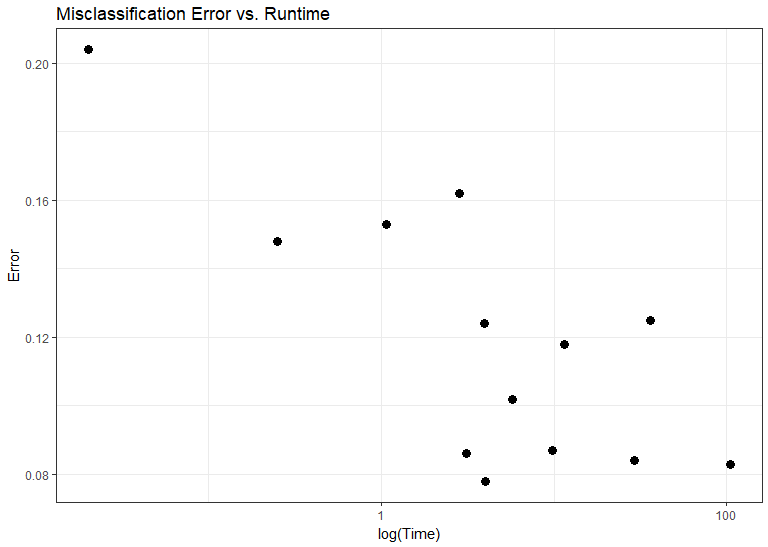
\includegraphics[scale=1]{plot}

\section*{Bibliography}

Eibe Frank, Mark A. Hall, and Ian H. Witten (2016). The WEKA Workbench. Online Appendix for "Data Mining: Practical Machine Learning Tools and Techniques", Morgan Kaufmann, Fourth Edition, 2016.



%\clearpage
%\newgeometry{top=1in, bottom=1in, left=0.5in}


\end{document}














